\ylDisplay{Satelliit} % Ülesande nimi
{Mihkel Pajusalu} % Autor
{piirkonnavoor} % Voor
{2011} % Aasta
{G 2} % Ülesande nr.
{1} % Raskustase
{
% Teema: Taevamehaanika
\ifStatement
Satelliit tiirleb ringikujulisel orbiidil (raadiusega $r=\SI{7000}{\kilo\metre}$) ümber maakera, kusjuures satelliidi orbiit on samas tasapinnas Maa orbiidiga ümber Päikese. Kui suure osa ajast veedab satelliit keskmiselt Maa varjus? Maa läbimõõt on $R=\SI{6378}{\kilo\metre}$. Päikeselt tulevad kiired võib lugeda paralleelseteks ja Maa liikumise ühe satelliidi orbiiditaalperioodi jooksul tühiseks.
\fi


\ifHint
Ringikujulisel orbiidil on satelliidi kiirus kogu orbitaalperioodi jooksul konstantne ja seetõttu on varjus veedetud osa ajast võrdne orbiidi varjus oleva osa pikkuse ja kogu orbiidi pikkuse suhtega.
\fi


\ifSolution
\begin{center}
	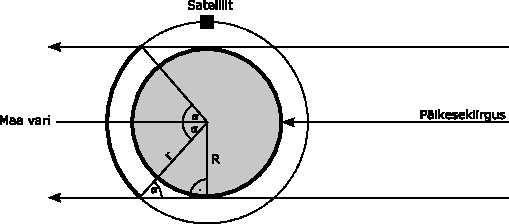
\includegraphics[width=0.9\linewidth]{2011-v2g-02-lah}
\end{center}
Ringikujulisel orbiidil on satelliidi kiirus kogu orbitaalperioodi jooksul konstantne ja seetõttu on varjus veedetud osa ajast võrdne orbiidi varjus oleva osa pikkuse ja kogu orbiidi pikkuse suhtega, mis on ülal toodud jooniselt leitav kui 
\[
k=\frac{2 \alpha r}{2 \pi r}=\frac{\arcsin \left(\frac{R}{r}\right)}{\pi}=\SI{36,5}{\%}
\]
\fi
}